\documentclass[a4paper]{scrartcl}
\usepackage[utf8]{inputenc}
\usepackage[english]{babel}
\usepackage{graphicx}
\usepackage{lastpage}
\usepackage{pgf}
\usepackage{wrapfig}
\usepackage{hyperref} 
\usepackage{fancyvrb}
\usepackage{fancyhdr}
\usepackage{float}
\pagestyle{fancy}

% Create header and footer
\headheight 27pt
\pagestyle{fancyplain}
\lhead{\footnotesize{Internet Applications, ID1354}}
\chead{\footnotesize{Linus Berg}}
\rhead{}
\lfoot{}
\cfoot{\thepage\ (\pageref{LastPage})}
\rfoot{}

% Create title page
\title{Linus' Fabulously Tasty cuisine!}
\subtitle{Internet Applications, ID1354}
\author{Linus Berg and linus@fenix.me.uk}
\date{Date}

\begin{document}

\maketitle

\section{Introduction}

\noindent The task was to create a recipe website that follow common web application design guidelines, and
learn HTML \& CSS while also learning the design patterns. Page layout; font size, family, and style;
foreground and background colour; mouse hovering and link behaviour, all of these things had to be
explicitly selected, and none may have the default value.\\\\
\noindent Certain pages were explicitly described for extra clarity.
\subsection{Index}
This is the front page of the web site, it shall be
informative and welcoming.  It shall promote
the calendar page and have a link to that page.

\subsection{Recipes}
There shall be one recipe page for each dish. In
this first version of the site, there are only two
dishes, meatballs and pancakes.  A recipe page
shall contain the name of the dish, an image
of the prepared meal, a list of ingredients, in-
structions and user comments. The user shall
not be able to write comments, instead  you
shall hard code sample comments.

\subsection{Calendar}
The calendar shall be a visual representation of one month, with clickable images of the
month’s dishes. These images shall be links to corresponding recipes. Your calendar
shall have dishes two days in the month, the meatballs day and the pancake day.

\section{Literature Study}
I was already quite familiar with all three technologies used (Javascript, HTML, CSS),
therefor a lot of literature studies could be skipped.
However W3C, Jquery API reference, Stackoverflow, and some sites were used for looking up
specific commands/tags.

\section{Method}

\noindent Explain how you worked when solving the tasks and how you evaluated that your solution met the requirements. Mention development tools and IDEs you used. \textit{Do not explain your solution and do not refer to code}, that belongs to the \textit{Result} section.
\\
The editor used for writing code was Vim, the rest of the software stack
utilised Python, Flask, and running all this was the WSGI server Gunicorn.\\\\
\textbf{Note:} If the server was to be facing 'outward' and accept public traffic, Nginx would
have been used as a reverse proxy to Gunicorn, however this was not part of the task.\\\\
The templating engine Jinja was used to 
make sure each page follows the same layout / structure,
this way was the most simple and frankly involved the least work.\\\\
This web stack was chosen because I am familiar with the whole process and my personal
opinions is that it is far superior to using a PHP solution as is used further in the course.\\\\
\noindent
The project started out with a simple website that adhered to all the requirements, however
it was extremely simple and bland, to avoid making just another website among thousands,
I decided to enjoy myself and do something unorthodox. I let the creative juices flow,
and made a comedic twist to the website while still displaying the required knowledge for
the lab (or at least I hope so).\\

\noindent
The development occured iteratively, gathering opinions on fonts, colours, and other
design choices, and fixed the issues accordingly. A lot of inspiration was drawn from
the 80's Outrun / Synthwave scene.
Scaling measurements (rem / \%) were also used to ensure website compatability.
Javascript was also extensively used to automatically generate HTML code, for easier portability.
\section{Result}
\begin{figure}[H]
  \begin{center}
    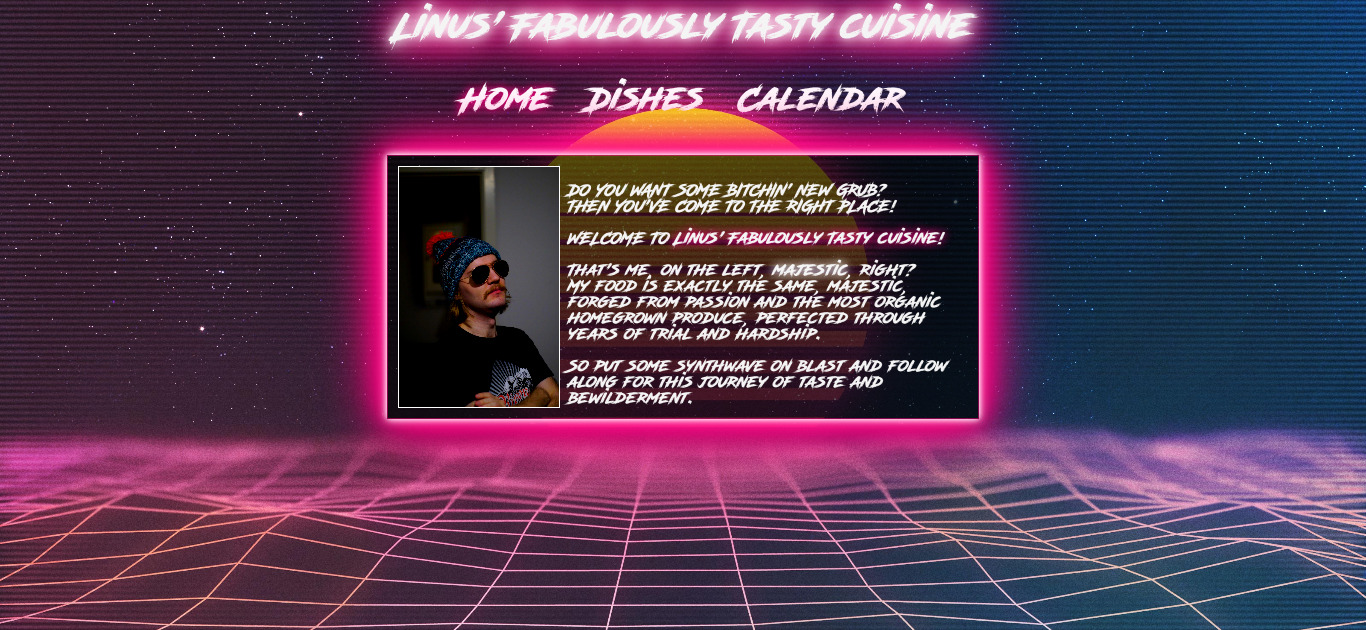
\includegraphics[scale=0.3]{Scr1.jpg}
    \caption{The inviting homepage!}
    \label{fig:homepage}
  \end{center}
\end{figure}

\begin{figure}[H]
  \begin{center}
    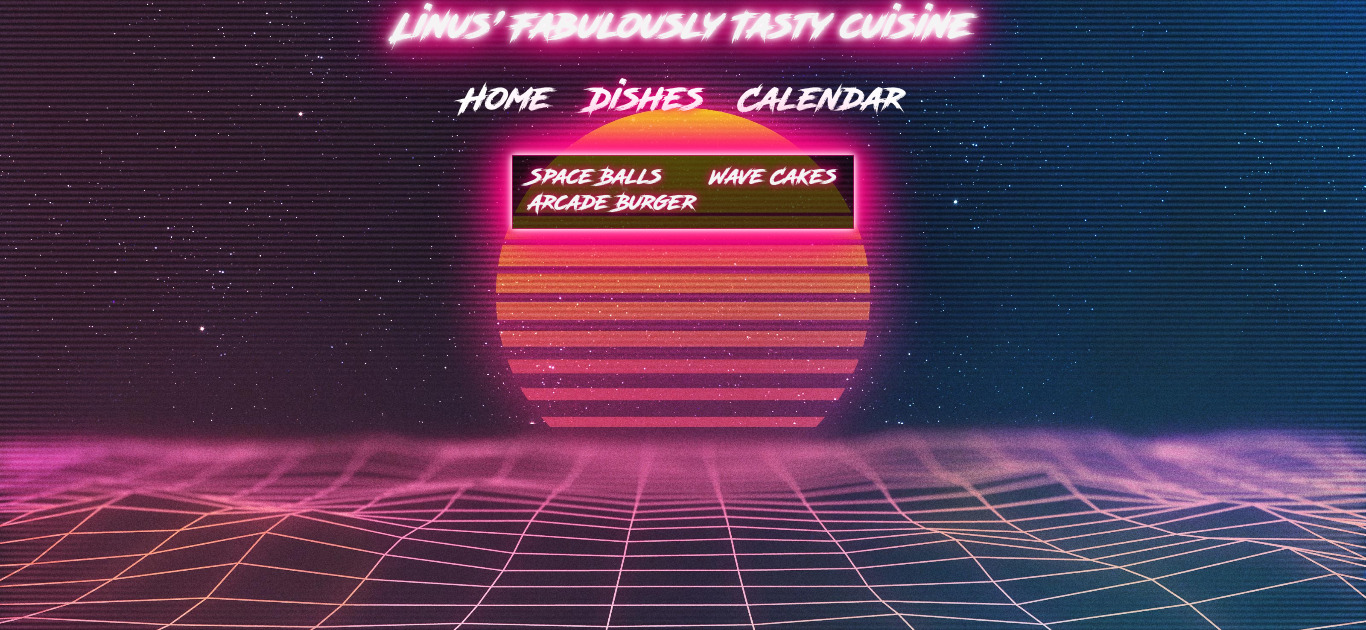
\includegraphics[scale=0.3]{Scr2.jpg}
    \caption{The pages displaying dishes available for the user to pick!}
    \label{fig:dishes}
  \end{center}
\end{figure}

\begin{figure}[H]
  \begin{center}
    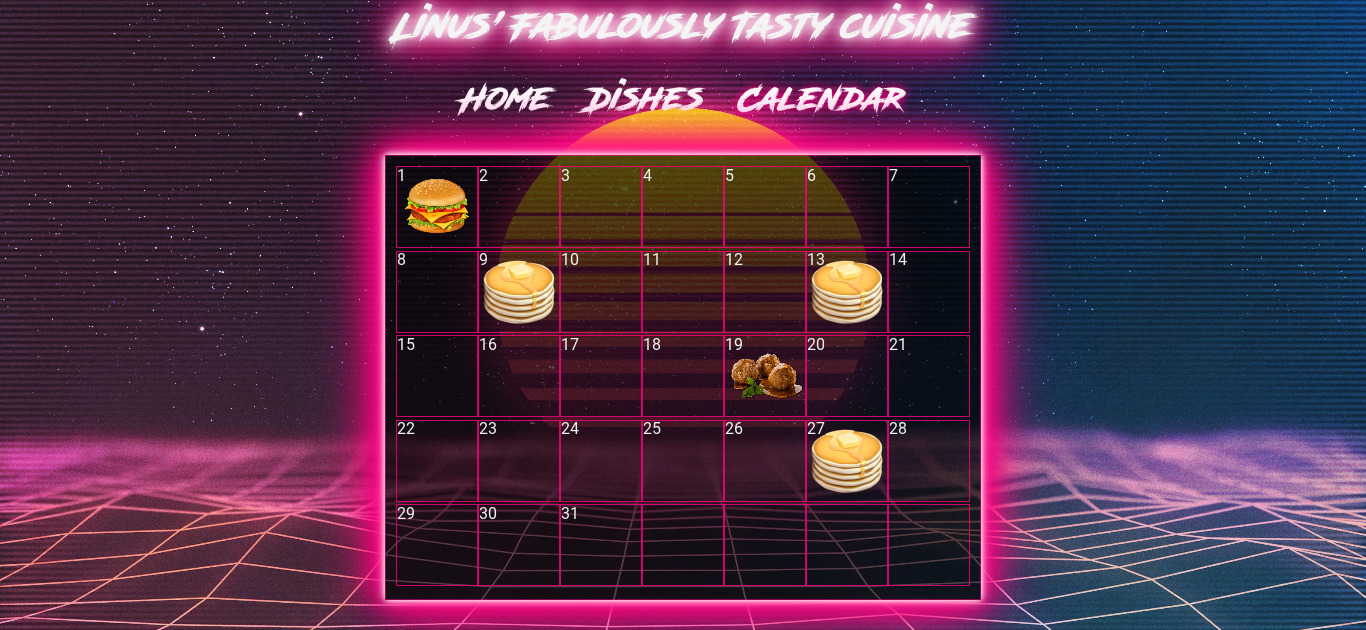
\includegraphics[scale=0.3]{Scr3.jpg}
    \caption{The dish calendar!}
    \label{fig:calendar}
  \end{center}
\end{figure}

\begin{figure}[H]
  \begin{center}
    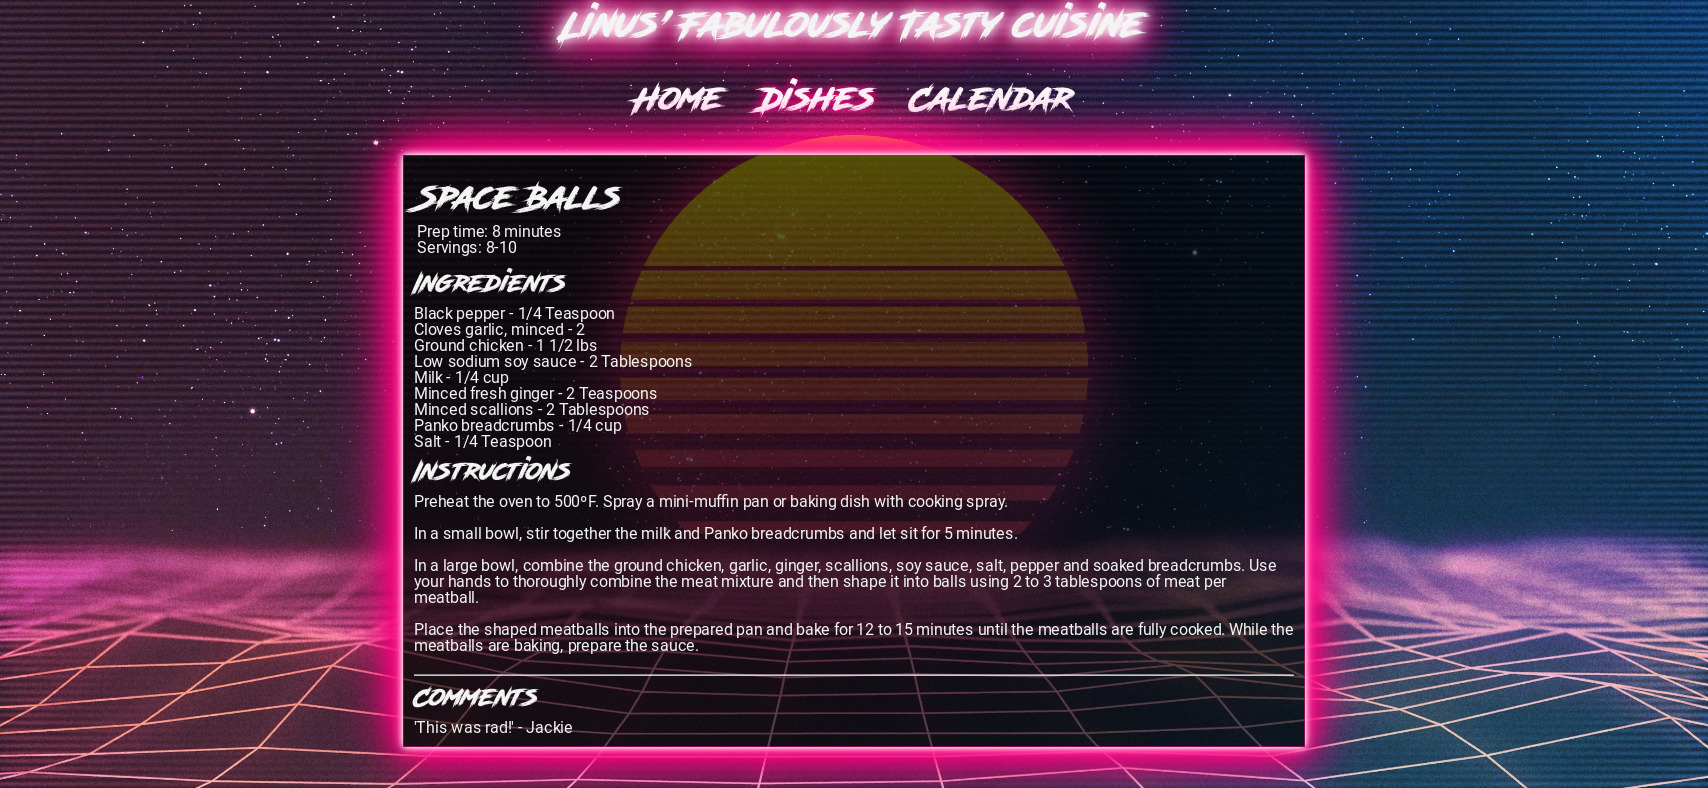
\includegraphics[scale=0.25]{Scr4.jpg}
    \caption{The recipe specification with comments!}
    \label{fig:recipe}
  \end{center}
\end{figure}
\begin{figure}[H]
  \begin{center}
    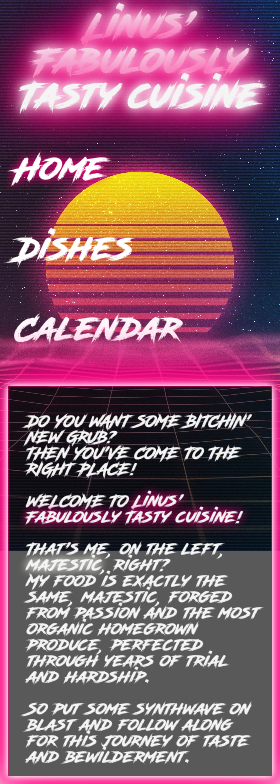
\includegraphics[scale=0.35]{Scr5.png}
    \caption{Example of mobile scaling!}
    \label{fig:recipe}
  \end{center}
\end{figure}
\begin{figure}[H]
  \begin{center}
    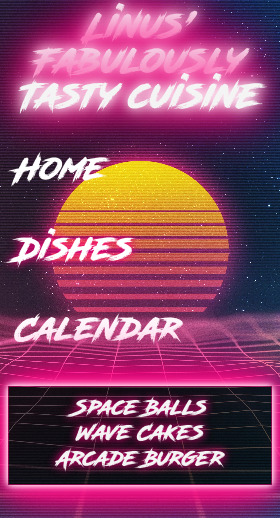
\includegraphics[scale=0.35]{Scr6.png}
    \caption{Example of mobile scaling!}
    \label{fig:recipe}
  \end{center}
\end{figure}
\newpage
\newpage
\noindent
\textbf{\href{https://github.com/linus-dev/KTH-Projects/tree/master/ID1354/1}{Github}}\\\\
The website should meet most of the requirements, however with own design choices implemented here and
there, such as no image is present in the specification of the recipe, however it is present in the
calendar, this was a concious choice. The following design patterns are however met.
\subsection{Visibility of system status}
This is not really that relevant to the website, however it conveys where the user
is currently browsing on the site by highligthing the navigation bar, see Figure \ref{fig:homepage}.
\subsection{Match between system and the real world}
No confounding language is used except some rad 80s slang (see Figure \ref{fig:homepage}),
the only thing that may be confusing for a user was the renaming of common dishes
to more align with the website theme.
\subsection{Consistency and standards}
The website has consistent naming of variables / classes / ids and pages, it also
adheres to the W3C standard (validation by the W3C validator was achieved).
\subsection{Recognition rather than recall}
The website is so simple the ordinary user should have no issues recognizing where to go,
and the project is too small to really drive this point home.
\subsection{Aesthetic and minimalist design}
This is the requirement the website strays from the norm the most, however
even though the design is quite outrageous, it is still quite aesthetically pleasing and
minimalistic (one of the reasons images was removed from the recipe specification).
The calendar however does not look that good and does not scale well, see Figure \ref{fig:calendar}.
\\\\
\noindent
The website was tested in several browsers and mobile devices, such as Firefox, Chrome, and Edge,
IE11 support is average at best, however it still displays, somewhat properly.
The site performs well on mobile devices as well, scaling decently, however some
pages could use some more work.
Overall the result is pleasing and light-hearted.
\newpage
\section{Discussion}
\noindent
I believe I met all the requirements with Aesthetic and minimalist design being the one failure.
The only problem I faced was laziness, for example, the calendar and other pages do not scale
brilliantly, especially the calendar, overall I believe I only spent around 4 hours building the site.\\\\

\noindent
The design could also have been better, a better / more fitting font could have been found for the
text on the front page, however this would require extensively searching for a fitting font,
something I deemed unecessesary for the task.\\\\

\noindent
The report template also states the code should be explained, however I found it diffcult
on these tasks to actually explain, as I am not sure which parts to explain.\\\\

\noindent
I could also have made a bland site for
pure functionality, but where is the fun in that?

\end{document}
